\documentclass[12pt]{article}
\setlength\parindent{0pt}
\usepackage{fullpage}
\usepackage{amsmath}
\usepackage{graphicx}
\setlength{\parskip}{4mm}
\def\LL{\left\langle}   % left angle bracket
\def\RR{\right\rangle}  % right angle bracket
\def\LP{\left(}         % left parenthesis
\def\RP{\right)}        % right parenthesis
\def\LB{\left\{}        % left curly bracket
\def\RB{\right\}}       % right curly bracket
\def\PAR#1#2{ {{\partial #1}\over{\partial #2}} }
\def\PARTWO#1#2{ {{\partial^2 #1}\over{\partial #2}^2} }
\def\PARTWOMIX#1#2#3{ {{\partial^2 #1}\over{\partial #2 \partial #3}} }
\newcommand{\BE}{\begin{displaymath}}
\newcommand{\EE}{\end{displaymath}}
\newcommand{\BNE}{\begin{equation}}
\newcommand{\ENE}{\end{equation}}
\newcommand{\BEA}{\begin{eqnarray}}
\newcommand{\EEA}{\nonumber\end{eqnarray}}
\newcommand{\EL}{\nonumber\\}
\newcommand{\la}[1]{\label{#1}}
\newcommand{\ie}{{\em i.e.\ }}
\newcommand{\eg}{{\em e.\,g.\ }}
\newcommand{\cf}{cf.\ }
\newcommand{\etc}{etc.\ }
\newcommand{\Tr}{{\rm tr}}
\newcommand{\etal}{{\it et al.}}
\newcommand{\OL}[1]{\overline{#1}\ } % overline
\newcommand{\OLL}[1]{\overline{\overline{#1}}\ } % double overline
\newcommand{\OON}{\frac{1}{N}} % "one over N"
\newcommand{\OOX}[1]{\frac{1}{#1}} % "one over X"



\begin{document}
\Large
\centerline{\sc{Homework 5}}
\normalsize
\centerline{\sc{Due Friday, 83 March}}

\begin{enumerate}


  \item A jet airplane is flying at a level course at constant speed; the engines are all running at maximum power. 

\begin{itemize}

\item What is the net force on the airplane?

\item Draw a force diagram of the plane as seen from the side with the plane
flying to the right. Name all of the forces shown on your diagram. 

\item Airplanes bank (tilt to the side) when they turn. Draw a force diagram of the 
plane as seen from behind as it turns to the left. 

\item Why do airplanes bank as they turn? Explain.
\end{itemize}

\item A heavy ball with mass 10 kg is hung from the ceiling of Stolkin Auditorium
on a rope of length 4.5 m. It is pulled to one side and released, swinging like
a pendulum; at its lowest point, it reaches a speed of 6 m/s. What is the tension
in the rope at that point?

  \item Astrologers claim that the positions of the planets can influence events on Earth. In this problem,
you'll calculate whether this is plausible or not.

\begin{enumerate}
\item Which planet's gravity do you think would have the greatest effect on Earth? Venus' orbit is closest,
but Jupiter is largest.
\item Look up astronomical parameters for Earth and your chosen planet. What is the closest they ever
are to each other? You may approximate their orbits as circles, and can find all the information you need
on Wikipedia. Show how you estimate their distance of closest approach.
\item What acceleration does your chosen planet impart to objects on Earth? Is this acceleration relevant 
to anything?
\end{enumerate}

\begin{minipage}{0.7\textwidth}
\item Two wires are tied to the sphere of mass 3 kg shown here. The sphere
revolves around the pole in a horizontal circle at constant speed.  

  \end{minipage}
  \begin{minipage}{0.3\textwidth}
\centerline{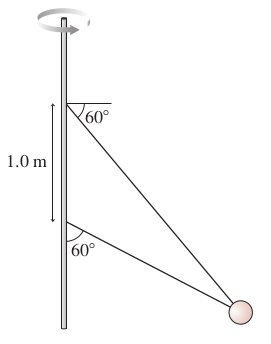
\includegraphics[width=0.9\textwidth]{problem837.png}}
  \end{minipage}

\begin{enumerate}
\item For what speed is the tension the same in both wires?
\item What is that tension?
\end{enumerate}

\item In class, you saw a demo consisting of a clear plastic tube of radius $r$ that rotated around its center. 
A pencil eraser of mass $m$ was placed against one of the walls of the tube, and the tube was spun.
If the coefficients of static and kinetic friction are $\mu_k$ and $\mu_s$, respectively, at what angular
velocity $\omega$ must the tube spin at for the eraser not to fall?

\item{

Merry and Pippin are sledding on the frozen surface of Lake Onondaga, which is quite close to a frictionless surface. Each of them plus his sled has a mass of 30 kg, but Merry also carries a stone that weighs 5 kg.
They are both traveling east at 2 m/s, right next to each other; Merry is north of Pippin. Merry throws his stone to Pippin, who catches it; the initial velocity of the stone is 5 m/s due south. (This means that Pippin may have to reach behind him a little bit to catch the stone, but that doesn't affect the problem.) Treat north as the positive $y-$axis and east as the
positive $x-$axis.

\begin{enumerate}
\item{What are the x and y components of Merry's velocity vector after he throws the stone?}
\item{What are the x and y components of Pippin's velocity vector after he catches the stone?}
\item{Initially, they had the same value of $v_x$. However, after one threw the stone and the other caught it, their $x-$velocities are different. Why is this? (Explain in words; no mathematics is required.)}
\end{enumerate}
}

\item{A clay block of mass 2 kg rests at the edge of a table of height 1 m. A bullet of mass 10 g is shot at it, 
striking the block at a speed of 500 m/s. The bullet sticks inside it, knocking the block off of the table. How far from the
edge of the table does it land?}


\item{A clay block and a steel block, each of mass 2 kg, sit on a table. The coefficient of friction between each of them and the table is 0.5.

Each of them is shot with a bullet of mass 3 g, traveling at a speed of 400 m/s. The bullet shot at the clay block lodges inside it, while the bullet 
shot at the steel block bounces off, traveling back in the direction that it came from at 200 m/s. 

\begin{enumerate}
\item{Without doing any mathematics, can you predict which block will slide further before coming to rest?}
\item{How far does the clay block slide?}
\item{How far does the steel block slide?}
\end{enumerate}
}

\item{\it (This problem is extra credit.) \rm A model rocket is pointed straight up and its motor ignited. The rocket accelerates upward at 20 $\rm m/\rm s^2$. The rocket has a mass of 1 kg.

The rocket motor consumes fuel at a rate of 15 grams per second, expelling 15 grams of gas out of the rear of the rocket at some exhaust velocity $v_e$ every second.

\begin{enumerate}
\item{What is the exhaust velocity $v_e$?}
{\it Hint:} Apply the impulse-momentum theorem to the exhaust gas; remember that for a constant force, $\Delta \vec p = \vec F t$. This will let you compute the relationship
between the exhaust velocity and the force that the rocket applies to the gas.
\item{The rocket's motor burns for 10 seconds before the fuel is exhausted. What is the acceleration of the rocket just before it runs out of fuel?}
{\it Hint:} The thrust force doesn't change, since it's the same rocket motor expelling fuel at the same rate. Why would the acceleration change once the rocket is
almost out of fuel?
\end{enumerate}


}

\item{An ambitious kestrel of mass 100 grams sees a tasty pigeon flying below it and dives to catch its dinner. The pigeon has a mass of 200 grams. It is flying horizontally at 
10 m/s when the kestrel, diving straight down, grabs it.

After the kestrel catches the pigeon, the two of them are moving in a direction 45 degrees below the horizontal. How fast was the kestrel moving before it caught the pigeon?}

\end{enumerate}



\end{document}
